\newcommand{\tabHBParams}{
%\newcolumntype{D}{>{\raggedleft\arraybackslash}m{0.65in}}
%\newcolumntype{E}{>{\raggedright\arraybackslash}m{2.75in}}
\newcolumntype{D}{>{\raggedleft\arraybackslash}m{0.6175in}}
\newcolumntype{E}{>{\raggedright\arraybackslash}m{2.7175in}}
\begin{table}[h]
  \centering
  %\vspace{-0.1in}
  \resizebox{0.7\linewidth}{!}{
  \begin{footnotesize}
    \begin{tabular}{DE}
      \toprule
      \textbf{Cores} & 128 cores in a 16x8 grid \\
      & RISC-V 32-bit IMAF ISA @ 1 GHz\\
      & 4KB Instruction Cache \\
      & 4KB Data Scratchpad \\ %%[.5ex]
      \midrule
      \textbf{Cache} & 128KB Total Capacity \\
      & 32 Independent Cache Banks \\
      & 8-way Set Associative\\ [.2ex]
      \midrule
      \textbf{NoC} & Bidirectional 2D Mesh NoC (32-bit data, 64-bit address) \\ [.2ex]
      \midrule
      \textbf{Memory} & 2 HBM2 memory channels \\
      & 32 GB/s per channel \\
      & 512 MB per channel \\
      \bottomrule
    \end{tabular}
  \end{footnotesize}
  }
  \caption{Configuration of the \hbmc used in this evaluation.}
  \label{tab:hbParams}
\end{table}
}

\newcommand{\hbBlockingEvalTab}{
\begin{table}[h]
\centering
\begin{footnotesize}
\begin{tabular}{lccc}
\toprule
\textbf{Graph} & \textbf{DRAM Stalls} & \textbf{Bandwidth} &  \textbf{Speedup} \\ \midrule
LiveJournal & 0.78 & 3.03 & 1.19    \\
Hollywood &  0.79 & 2.17 & 1.53   \\
Pokec & 0.83 & 3.02 & 1.49     \\
\bottomrule
\end{tabular}
\end{footnotesize}
  \caption{Impact of the blocked access optimization on SSSP. Reduction in DRAM stalls, improvement in memory bandwidth utilization, and overall speedup. } %over the unoptimized version of \sssp. }%Results are shown for the three graphs for which the blocked access method was the optimal schedule.}
\label{tab:hb_blocking}
\end{table}
}

\newcommand{\edgeAwareHist}{
\begin{sidewaysfigure}
    \centering
    \subfloat[BFS 18]{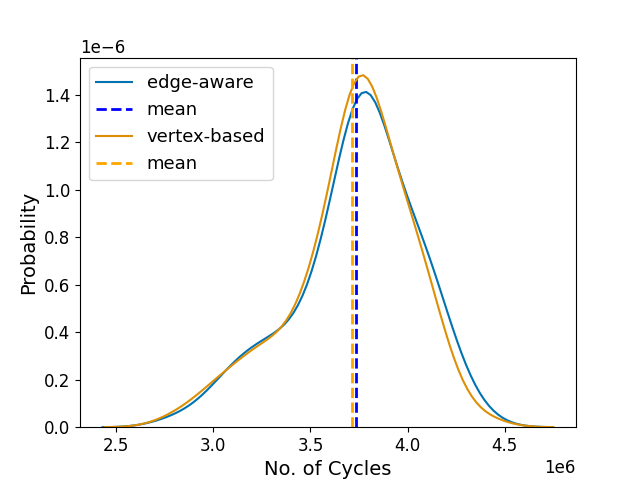
\includegraphics[width=0.3\textwidth]{graphit-figures/bfs-pull-18-edge-aware.png}}
    \subfloat[BFS 19]{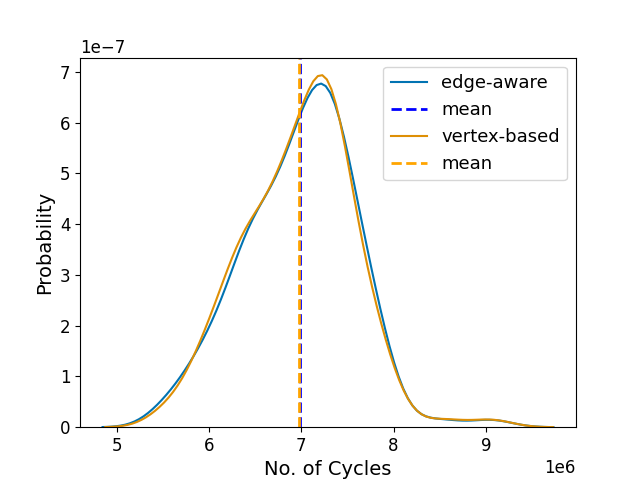
\includegraphics[width=0.3\textwidth]{graphit-figures/bfs-pull-19-edge-aware.png}}
    \subfloat[BFS 20]{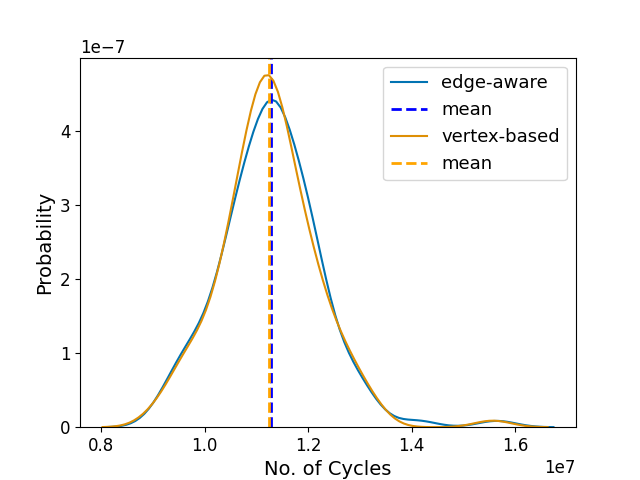
\includegraphics[width=0.3\textwidth]{graphit-figures/bfs-pull-20-edge-aware.png}} \\
    \subfloat[SSSP 18]{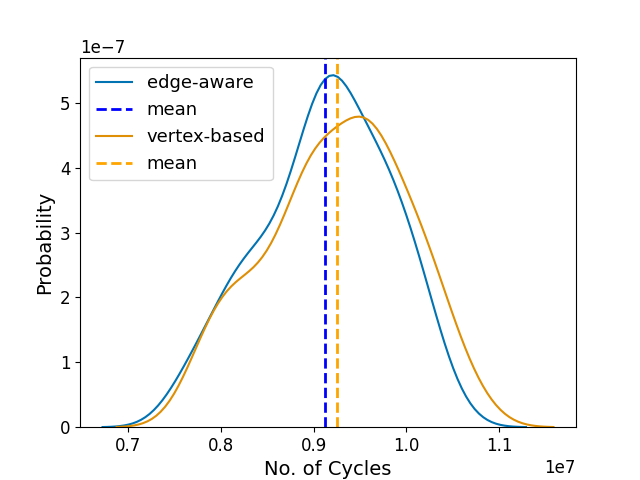
\includegraphics[width=0.3\textwidth]{graphit-figures/sssp-pull-18-edge-aware.png}}
    \subfloat[SSSP 19]{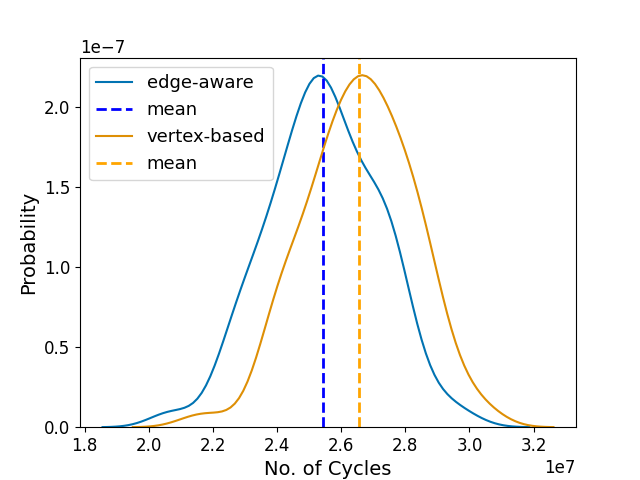
\includegraphics[width=0.3\textwidth]{graphit-figures/sssp-pull-19-edge-aware.png}}
    \subfloat[SSSP 20]{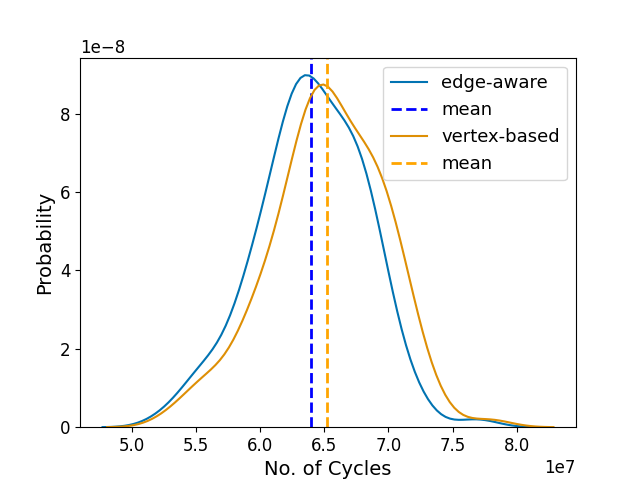
\includegraphics[width=0.3\textwidth]{graphit-figures/sssp-pull-20-edge-aware.png}} \\
    \subfloat[PR 18]{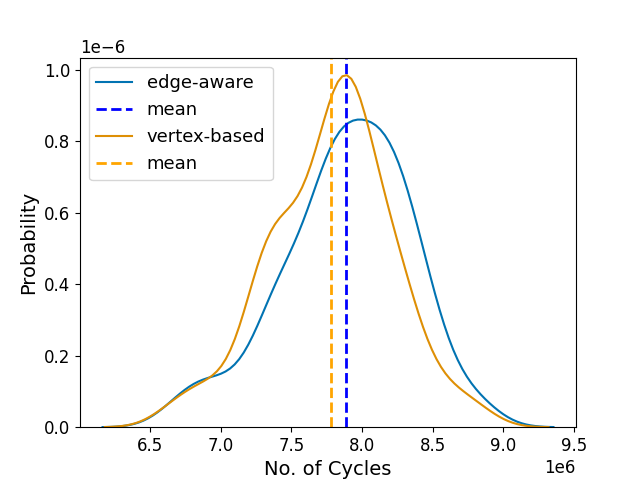
\includegraphics[width=0.3\textwidth]{graphit-figures/pr-pull-18-edge-aware.png}}
    \subfloat[PR 19]{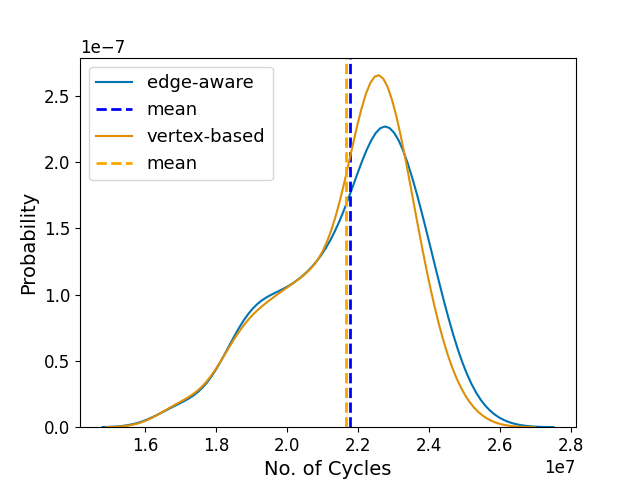
\includegraphics[width=0.3\textwidth]{graphit-figures/pr-pull-19-edge-aware.png}}
    \subfloat[PR 20]{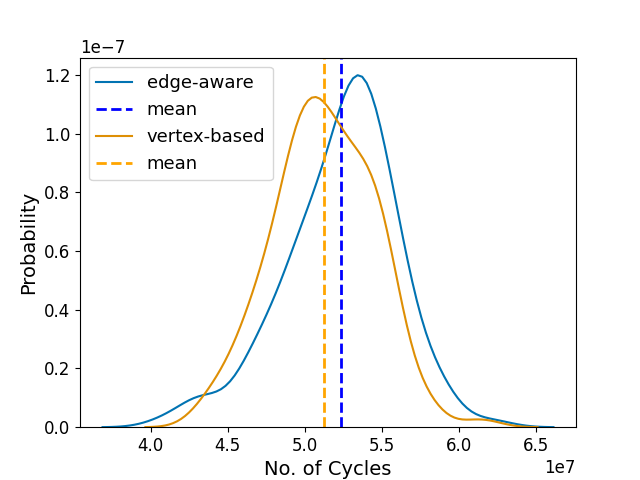
\includegraphics[width=0.3\textwidth]{graphit-figures/pr-pull-20-edge-aware.png}}
    \caption{Probability distribution of cycle counts for each core for vertex-based and edge-aware partitioning.}
    \label{fig:load_balance:cycledist}
\end{sidewaysfigure}
}

\newcommand{\alphatune}{
  \begin{figure}[h!]
    \centering
    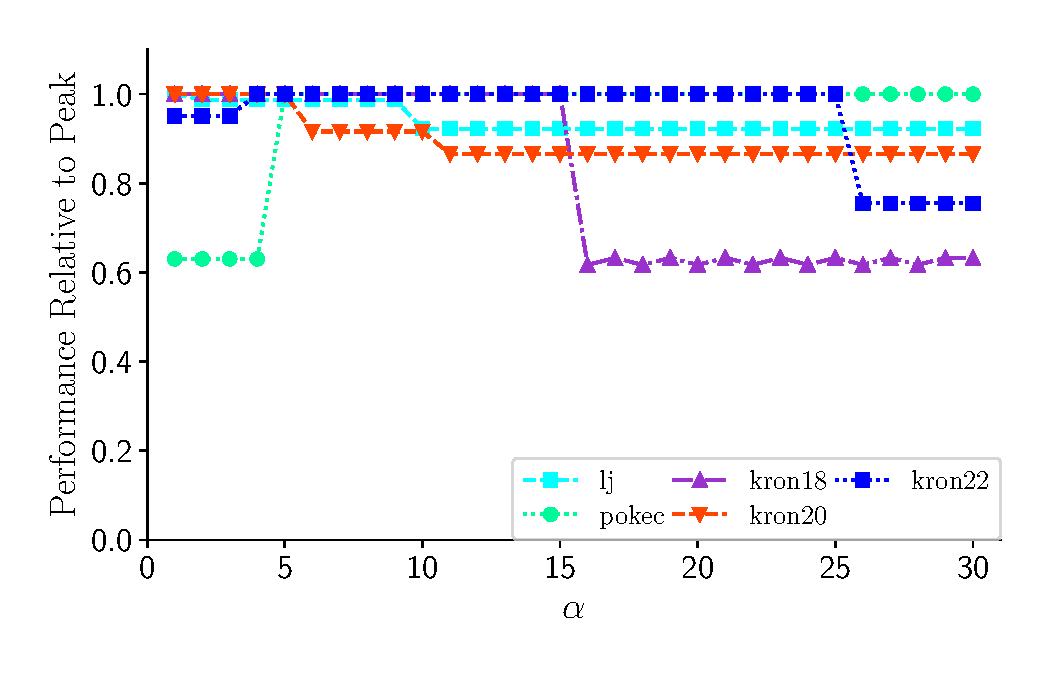
\includegraphics[scale=0.6]{graphit-figures/alpha.pdf}
    \caption{Performance results for hybrid traversal on BFS for each graph relative to its best performance for a range of $\alpha$ values. We find $\alpha = 5$ to be optimal on \hb.}% \todo{finish caption}}
    \label{fig:alpha_tuning}
  \end{figure}
}

\newcommand{\betatune}{
  \begin{figure}[h!]
    \centering
    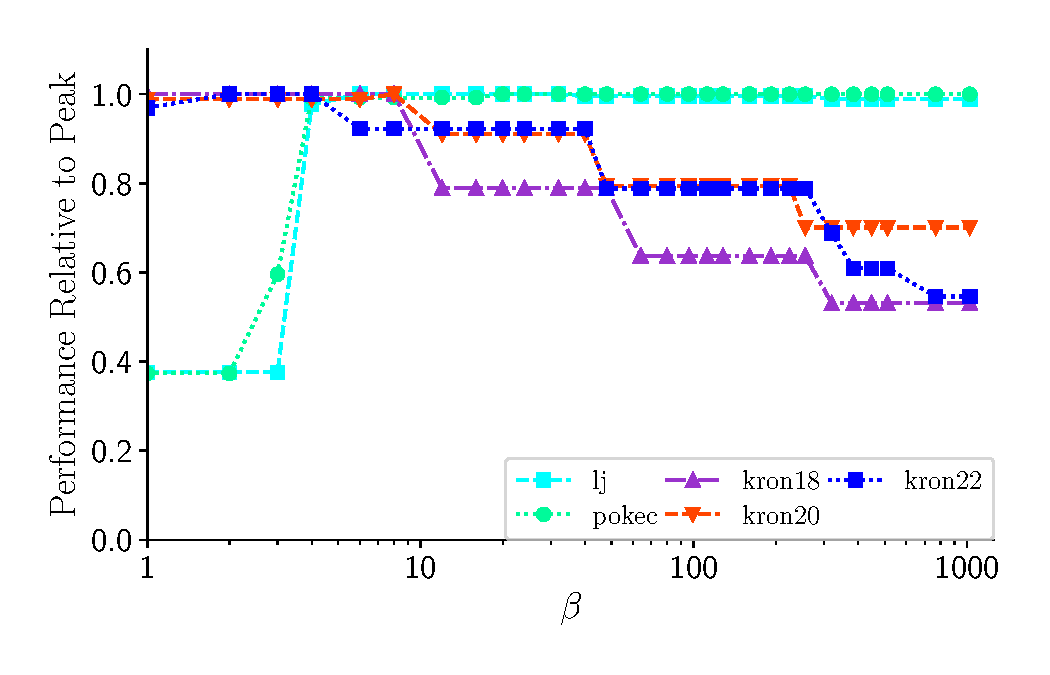
\includegraphics[scale=0.6]{graphit-figures/beta.pdf}
    \caption{Performance results for hybrid traversal on BFS for each graph relative to its best performance for a range of $\beta$ values. We find $\beta = 4$ to be optimal for these graphs on \hb}% \todo{finish caption}}
    \label{fig:beta_tuning}
  \end{figure}
}

\newcommand{\hybridresults}{
  \begin{figure}[h!]
    \centering
    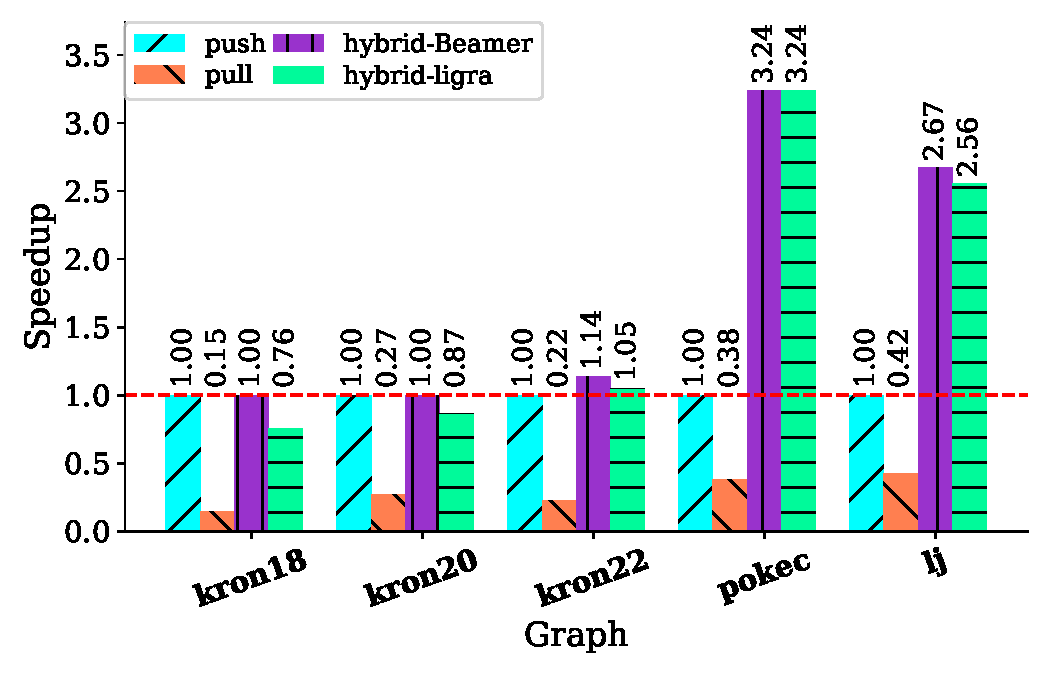
\includegraphics[scale=0.6]{graphit-figures/hybrid-dir.pdf}
    \caption{Traversal direction speedups for BFS relative to the \push implementation. Hybrid-beamer is the hybrid method proposed by Beamer et al. and hybrid-ligra is the method introduced in Ligra.}
    \label{fig:hybrid_dir}
  \end{figure}
}